\documentclass[dvipdfmx,autodetect-engine, 12pt]{jsarticle}

\usepackage{ulem} % 取消線を引くためのパッケージ
\usepackage[dvipdfmx]{graphicx} % 画像を挿入するためのパッケージ
\usepackage{array} % 表の幅指定や自動改行に必要
\usepackage{enumitem}

% --- 考文献用の設定 ---
\usepackage[backend=biber, style=numeric]{biblatex} % biblatexパッケージの使用
\addbibresource{report3.bib} % 先ほど作った別ファイルを指定（拡張子まで書く）
\usepackage{url} % WebサイトのURLを綺麗に出力するため

% --- section の文字サイズを小さくする設定 ---
\makeatletter
\renewcommand{\section}{%
  \@startsection{section}{1}{\z@}%
  {1.5ex \@plus .5ex \@minus .2ex}% 前の行との隙間
  {0.5ex \@plus .3ex}% 下の行との隙間
  {\normalfont\normalsize}% ← ここでサイズを \Large（少し大きめ）に指定
}
\makeatother

\begin{document}

% 課題のタイトル
\begin{center}

    {\LARGE \bfseries 課題③\,ARPおよびICMPパケットの解析\par}

\end{center}

\vspace{1cm}

{\LARGE \uline{目的}} 

\vspace{1cm}

{\LARGE \uline{事前準備}} 

\begin{enumerate}
    \item server と router の VM を起動する．
    \item arp と ping コマンドで利用されるプロトコルを調査する.
\end{enumerate}

\vspace{1cm}

{\LARGE \uline{手順}} 

\begin{enumerate}
    \item arpとpingコマンドで, どのプロトコルが利用されるのか調査し, 
          特に通信の開始から終了までに, 通信元と通信先との間に, OSI参照モデルのどの層で, 
          どのような手順で, どのように, どのような情報が, やり取りされるのか詳細を調べ, 整理しなさい.

        \vspace{\baselineskip}

        \quad arpコマンドは, ARP(Address Resolution Protocol)によって, ARPテーブルに記録された情報を表示・編集するためのコマンドである\cite{bashdo_arp}.
        ARPとは, ネットワークがコンピュータのIPアドレスと物理的なマシンアドレスを変換（解決）するために使用される一般的な手法であり\cite{kinsta_arp}, 
        宛先ホストのIPアドレスを手がかりに, 次に送るべき機器のMACアドレスを調べる.
        送信元IPアドレスと宛先IPアドレスを比較して, 宛先IPアドレスが同じネットワーク上にあるときには, その宛先IPアドレスのMACアドレスを調べ, 
        宛先IPアドレスが異なるネットワーク上にある場合には, 次に送るルータのIPアドレスからMACアドレスを調べる.
        ARPパケットのフォーマットと各フィールドの説明をそれぞれ図\ref{fig:arp_packet_format}と表\ref{tab:arp_fields}に示す.
        \\
        

        \begin{figure}[htbp]
            \centering
            % [width=...] で画像の横幅を調整します（例: 紙幅の80%）
            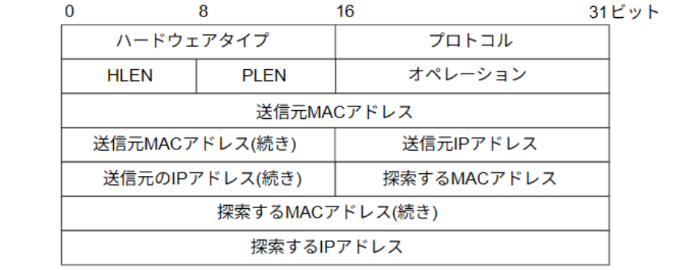
\includegraphics[width=0.8\textwidth]{imgs/arp_packet_format.png} 

            % 図の下に表示されるキャプションと引用
            \caption{ARPによるアドレス解決の仕組み（\cite{nw_text_r08}より引用・改変）}

            % 本文から「図1」として呼び出すためのラベル（captionの直後に書く）
            \label{fig:arp_packet_format}
        \end{figure}

        \begin{table}[htbp]
            \centering
            \caption{ARPパケットのフィールド構成（\cite{nw_text_r08}を参照に作成）}
            \label{tab:arp_fields}
            % p{8cm} を m{8.5cm} に変更し、垂直方向の中央揃えと幅の調整を行います
            \begin{tabular}{|c|c|m{8.5cm}|}
                \hline
                \multicolumn{1}{|c|}{フィールド名} & ビット数 & \multicolumn{1}{c|}{内容} \\ \hline
                ハードウェアタイプ & 16 & どのようなデータリンクを使用しているかを示す． \\ \hline
                プロトコルタイプ   & 16 & ネットワーク層のプロトコルについて示す． \\ \hline
                HLEN              & 8  & ハードウェアアドレスの長さを示す． \\ \hline
                PLEN              & 8  & プロトコルアドレスの長さを示す． \\ \hline
                オペレーション     & 16 & ARP要求パケットかARP応答パケットかを示す．\newline ARP要求パケットの場合は1，\newline ARP応答パケットの場合は2． \\ \hline
                \begin{tabular}{@{}c@{}}送信元MAC\\アドレス\end{tabular}  & 48 & 送信元MACアドレスを示す．\newline ARP応答パケットでは，ここにARP要求パケットで求めていたMACアドレスが設定されて返される． \\ \hline
                \begin{tabular}{@{}c@{}}送信元IP\\アドレス\end{tabular}   & 32 & 送信元IPアドレス． \\ \hline
                \begin{tabular}{@{}c@{}}探索するMAC\\アドレス\end{tabular} & 48 & 探索するMACアドレスを示す．ARPパケットではここが分からないので，通常は0の値が設定されている． \\ \hline
                \begin{tabular}{@{}c@{}}探索するIP\\アドレス\end{tabular}  & 32 & ARP要求パケットでは，探索するIPアドレスを示し，ARP応答パケットでは，宛先（要求パケットの送信元）のアドレスが設定される． \\ \hline
            \end{tabular}
        \end{table}

        \quad 続いて, ARPによってアドレス解決を行う際の手順について示す.
        ここではホストAがホストBのMACアドレスを解決しようとしているものとする.

        \vspace{\baselineskip}

        \begin{enumerate}[label=\textcircled{\scriptsize\arabic*}]
            \item ホストAは探索するIPアドレスにホストBのIPアドレスを指定したARP要求パケットをネットワークにブロードキャストする.
            \item ホスト B は ARP 要求パケットを受け取ると, ホスト A に対して自身の NIC に割り当てられている MAC アドレスを ARP ユニキャストする.
            \item ホスト A は ARP 応答パケットを受け取り, そこに記述される MAC アドレスはコンピュータ内の ARP テーブルに登録され, 数分間キャッシュされる. 一度登録されるとキャッシュされている間は ARP の再問い合わせが実行されることはない.
        \end{enumerate}


\end{enumerate}

\newpage

% --- 参考文献リストの出力 ---
\printbibliography[title=参考文献]

\end{document}